\documentclass[aps,pre,superscriptaddress]{revtex4}

\usepackage{preamble}
\graphicspath{ {./figures} }

\begin{document}

% \begin{abstract}
% \end{abstract}

\title{SBM-WCC Ian's Document}
\author{Ian Chen}
\noaffiliation
\date{\today}
\maketitle

\section{Introduction}
See the preprint~\cite{Park25-02}.

\section{Materials and Methods}

We used 122 networks --- 120 networks from the Netzschleuder network catalogue~\cite{Netzschleuder} and two other networks from ~\cite{Park24-11}.
The networks range in size, from 11 to 13,989,436 nodes, and 13 to 117,185,083 edges.

On two networks (libimseti and epinions), the analysis did not work? 
Need to check this, maybe rerun (blank output file?).

\section{Nested-SBM on Empirical Networks}

\begin{figure}
	\centering
	\begin{subfloat}
		\centering
		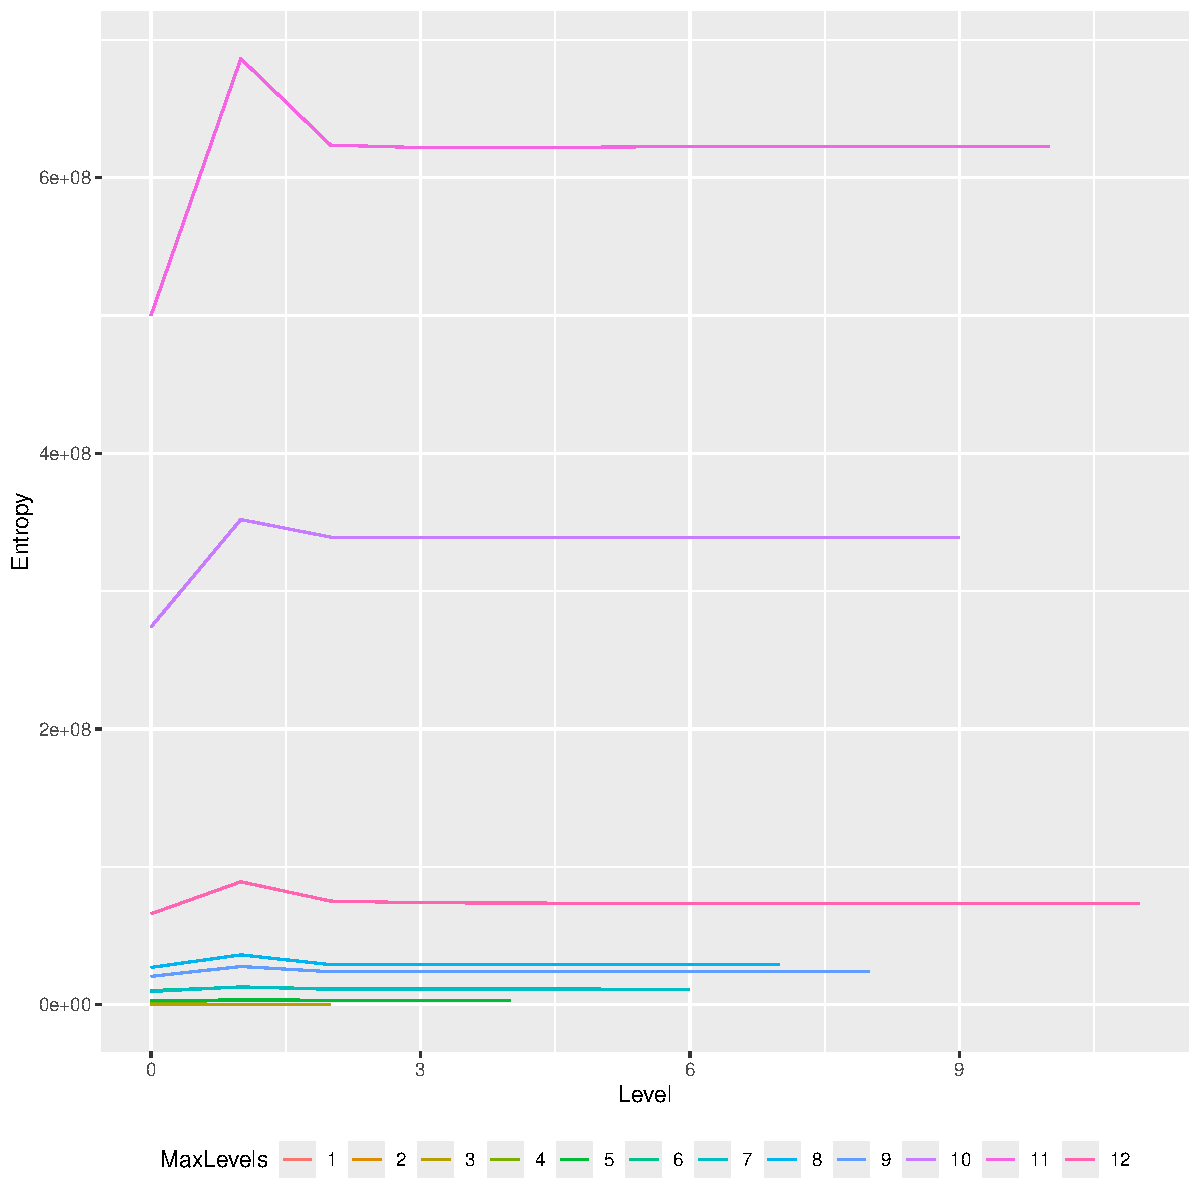
\includegraphics[width=0.48\textwidth]{fig1.pdf}
	\end{subfloat}
	\begin{subfloat}
		\centering
		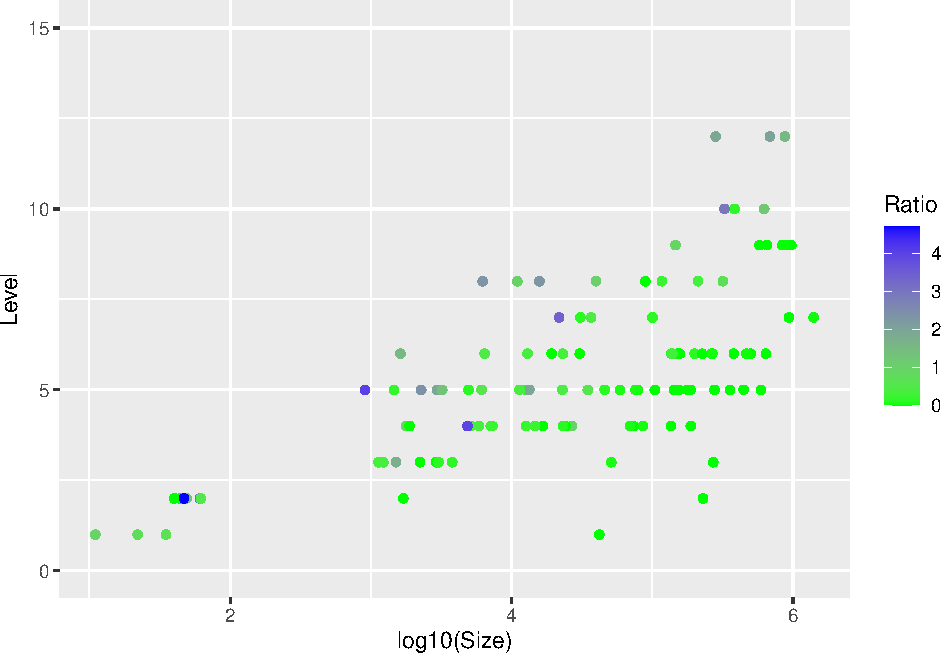
\includegraphics[width=0.48\textwidth]{fig2.pdf}
	\end{subfloat}
	\caption{Entropy and Clusters across Hierarchical-SBM Levels:
		On all empirical networks (120).
		For each plot, we take the mean across all networks with MaxLevels number of inferred levels.
		Left: The description length is calculated according to the Degree Corrected (non-nested) SBM model.
		Right: The number of clusters (log scale).
	}
	\label{figs:fig1}
\end{figure}

\begin{figure}[ht]
	\centering
	\begin{subfloat}
		\centering
		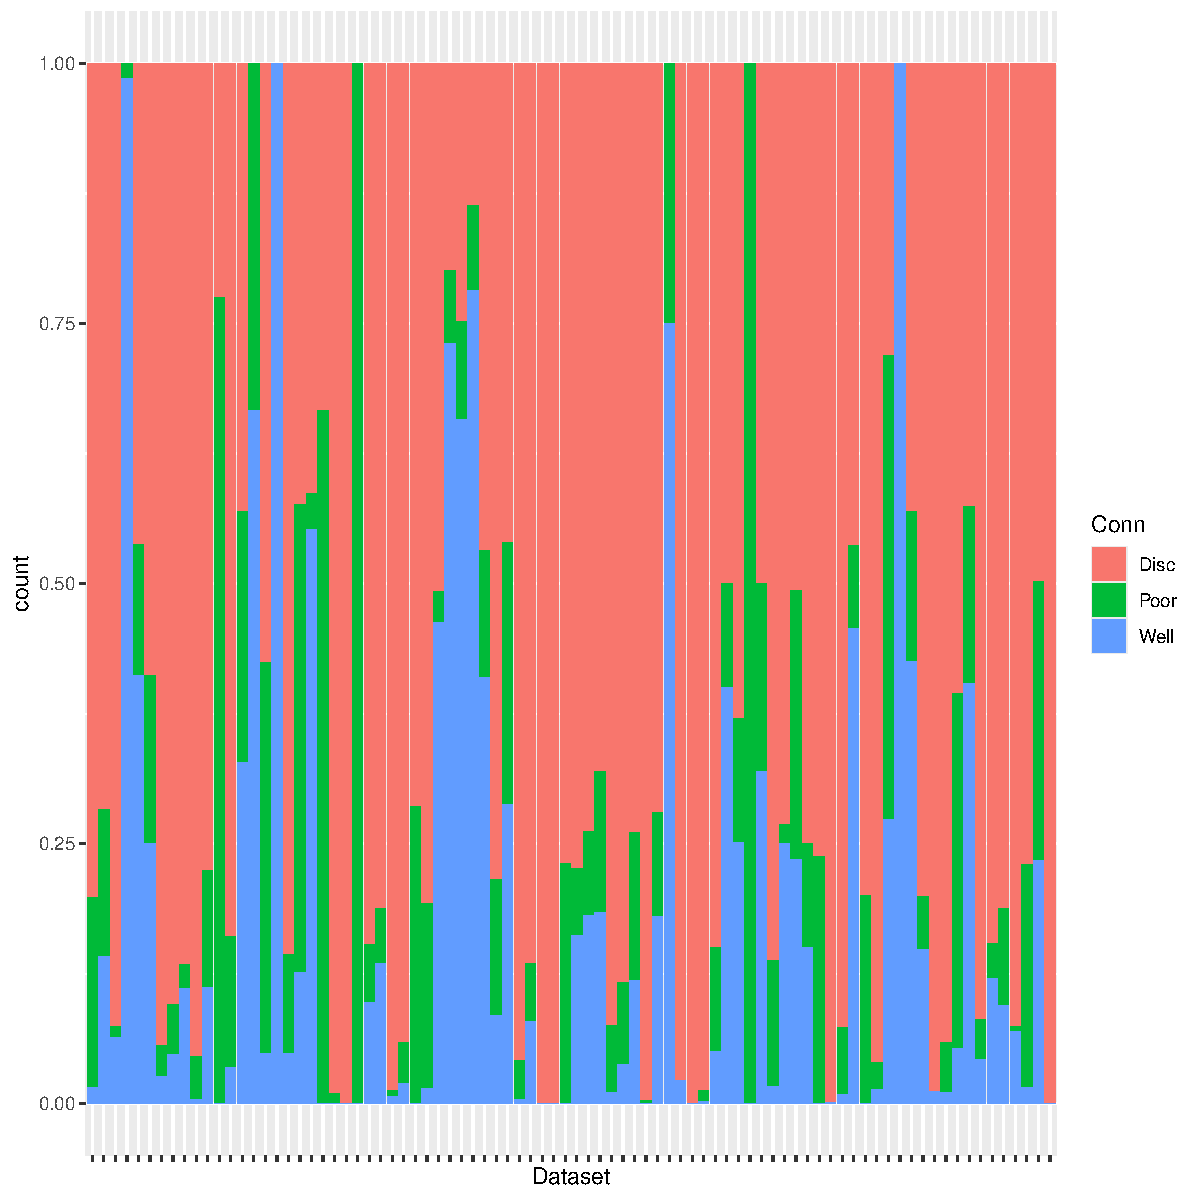
\includegraphics[width=0.4\textwidth]{fig3a.pdf}
	\end{subfloat}
	\begin{subfloat}
		\centering
		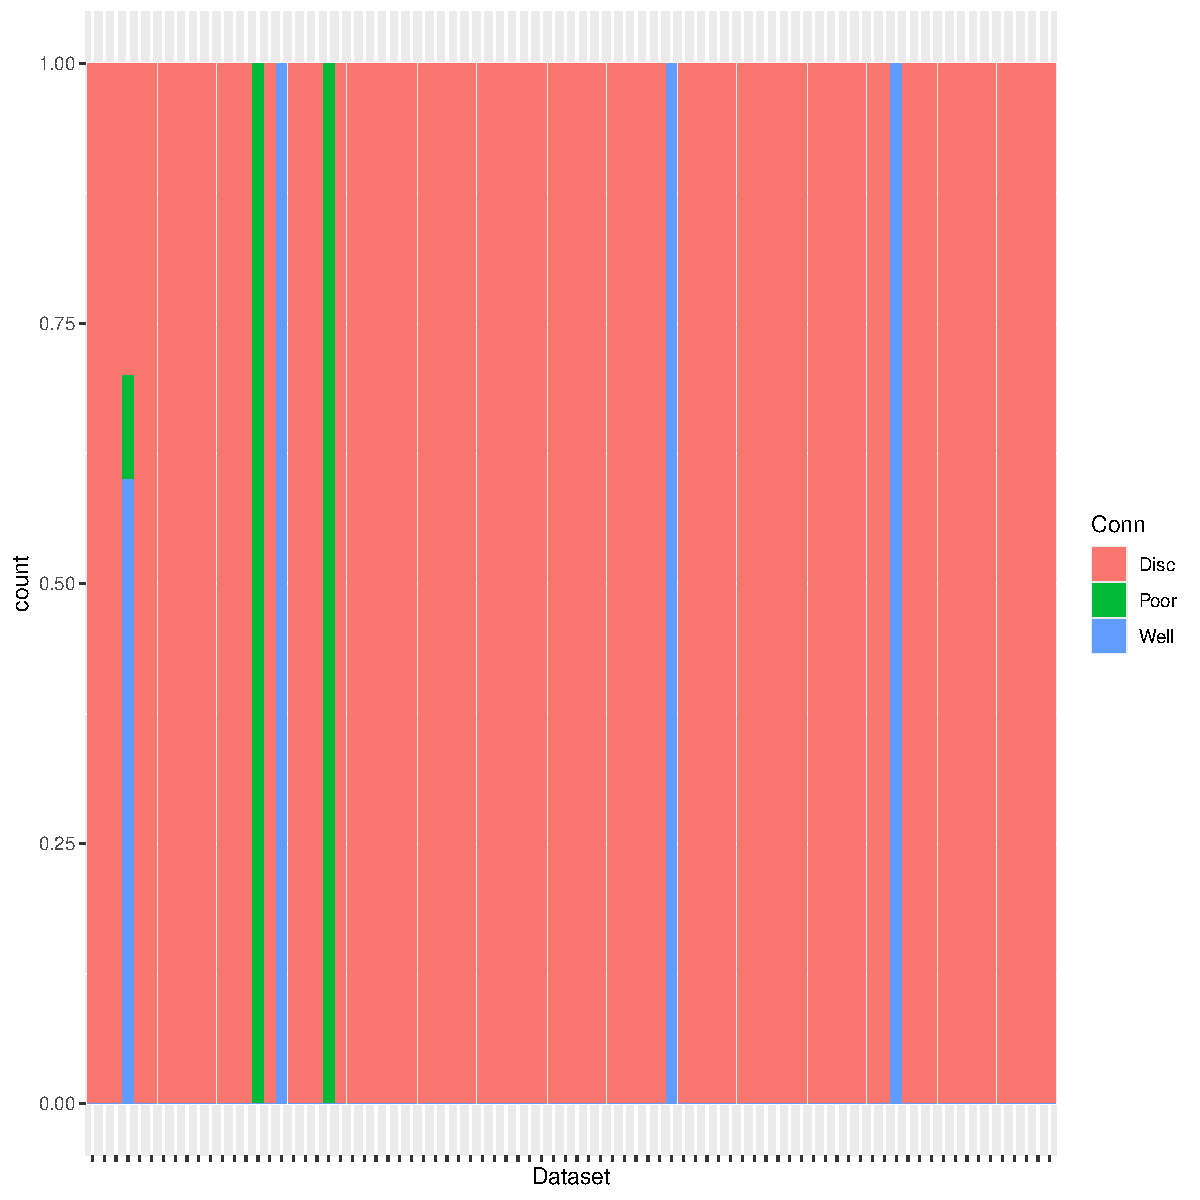
\includegraphics[width=0.4\textwidth]{fig3b.pdf}
	\end{subfloat}
	% \begin{subfloat}
	% 	\centering
	% 	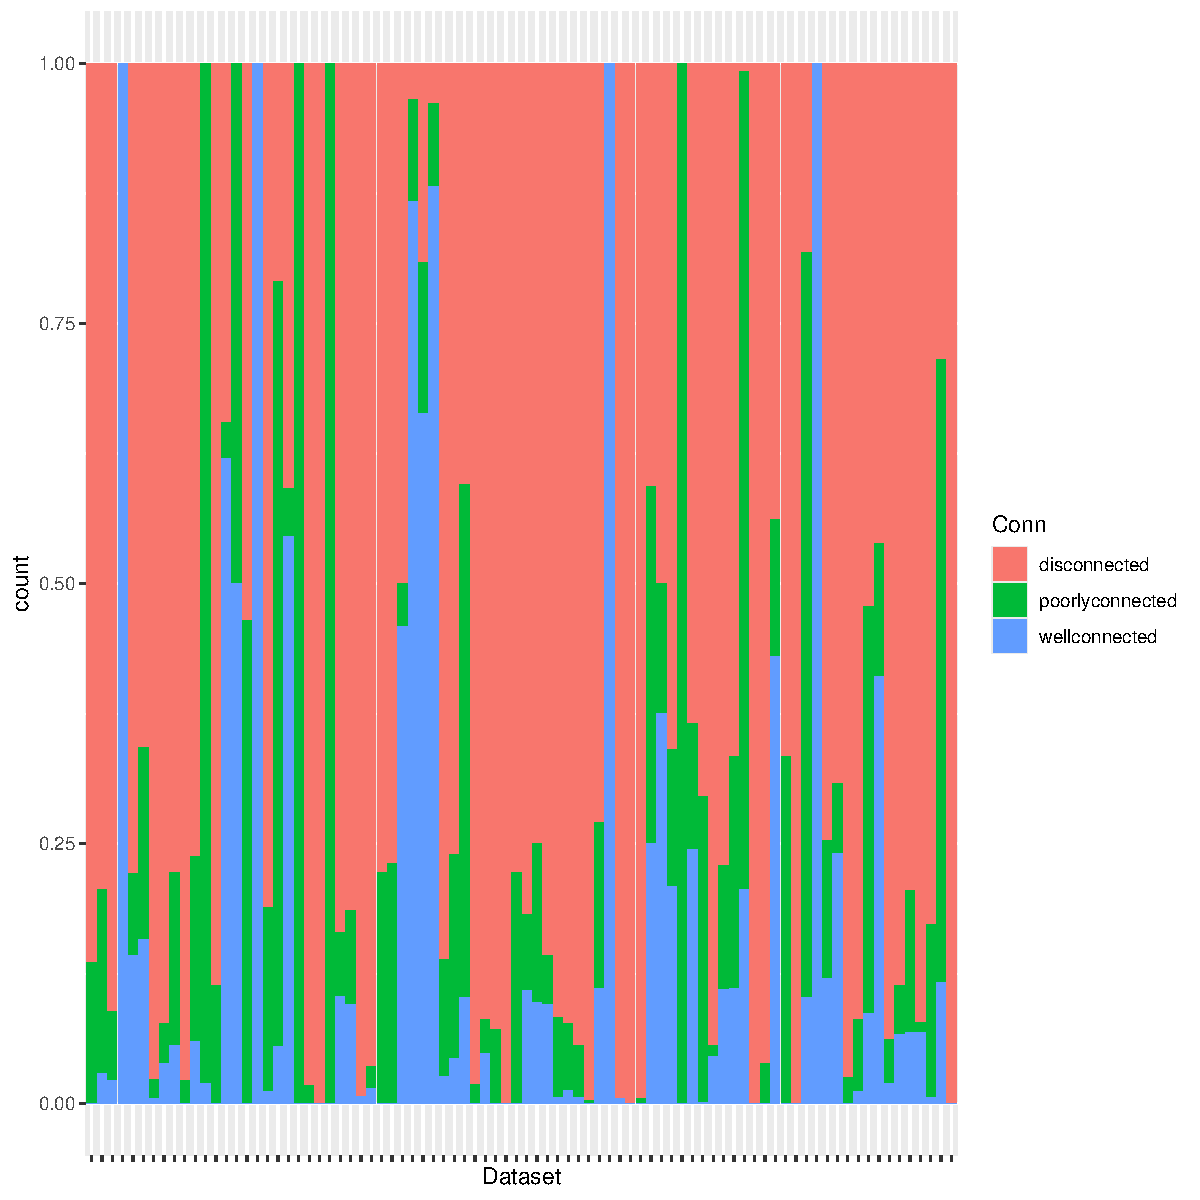
\includegraphics[width=0.8\textwidth]{fig3c.pdf}
	% \end{subfloat}
	\caption{Connectivity of Hierarchical-SBM Clusters.
		On the non-bipartite empirical networks (86).
		Each bar is a network, sorted in increasing network size.
		The y-axis shows percentage disconnected, poorly-connected $\setminus$ disconnected, and well-connected
		(a) Level0 (b) Level1}
	\label{figs:fig2}
\end{figure}

\begin{figure}[ht]
	\centering
	\begin{subfloat}
		\centering
		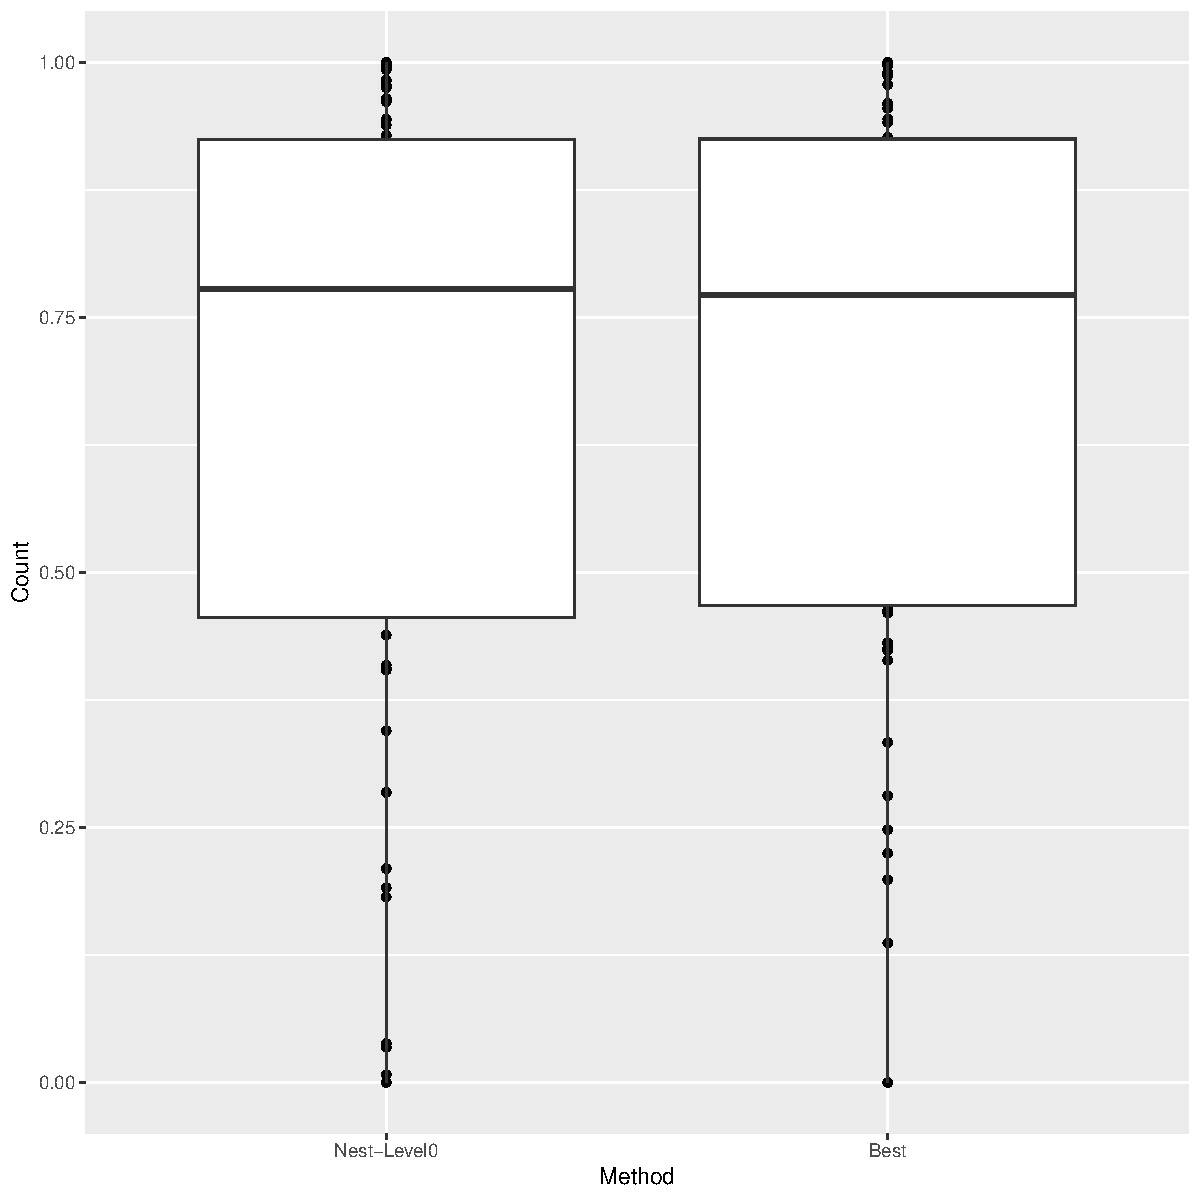
\includegraphics[width=0.4\textwidth]{fig4a.pdf}
	\end{subfloat}
	\begin{subfloat}
		\centering
		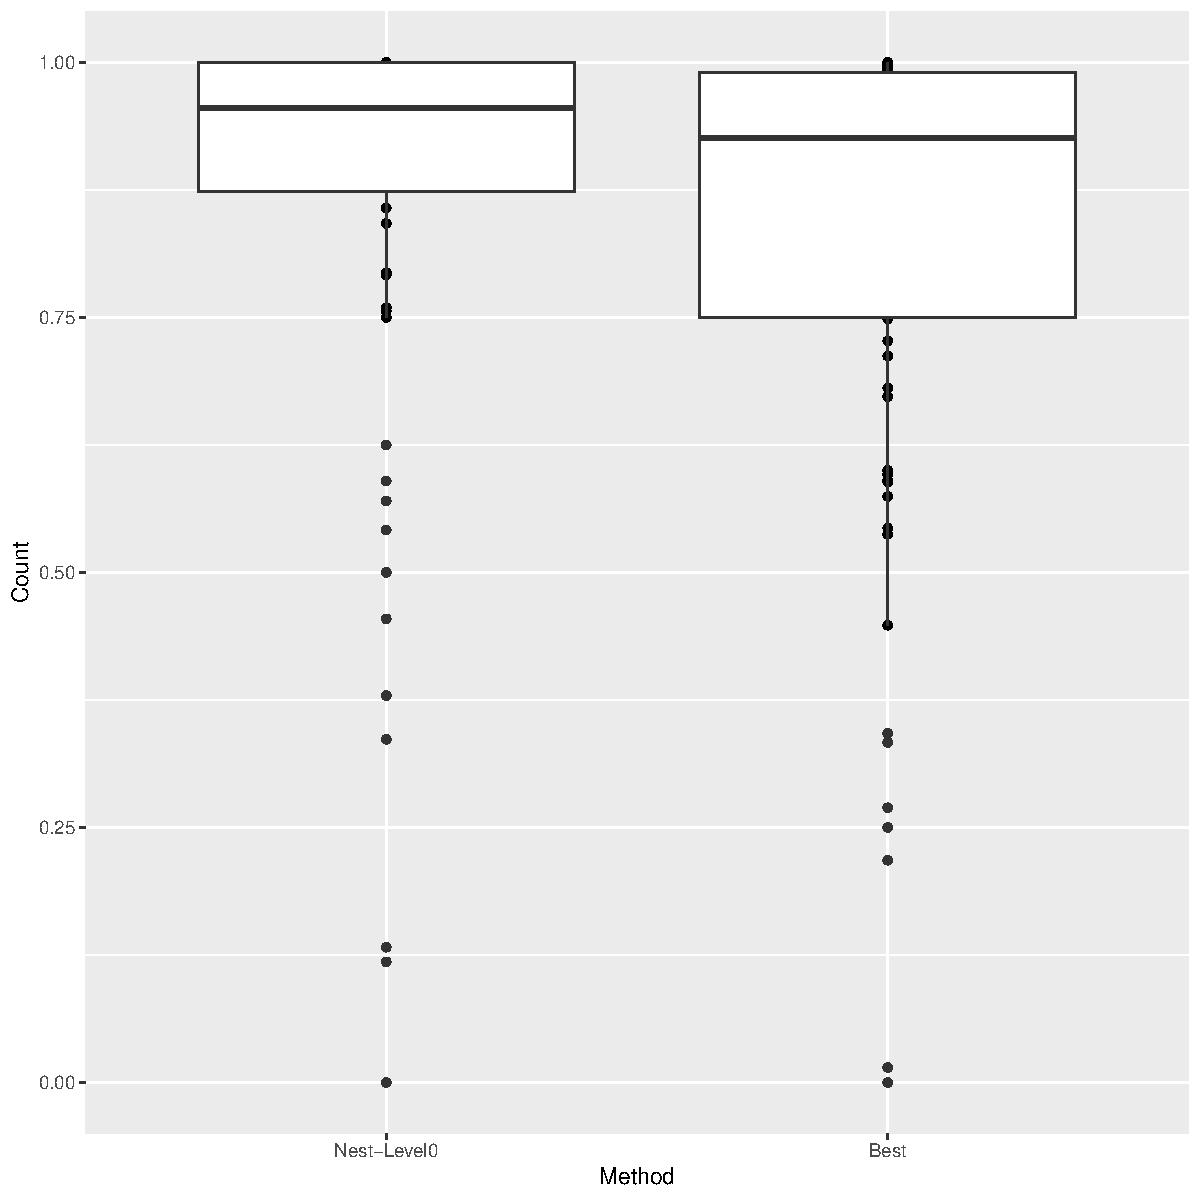
\includegraphics[width=0.4\textwidth]{fig4b.pdf}
	\end{subfloat}
	\caption{Connectivity Comparison:
		On the non-bipartite empirical networks (86).
		We calculate the percentage of disconnected clusters and compare with the hierarchical (left) and the non-hierarchical (right).
	}
	\label{figs:fig3}
\end{figure}

On average, the best layer by itself (via description length) is Layer 0 (Figure \ref{figs:fig1}).
Moreover, on all the 120 empirical networks (except for petster), the layer with the lowest description length (compared to the other layers) is Layer 0 --- on petster, it was layer 4 (out of 10 layers).

Conducting a paired t-test of disconnected percentages, there is no statistical difference between disconnected percentage (p = 0.5264).
However, comparing the poorly-connected percentage, there is a statistical difference (p = 0.0193).

\section{PySBM}

\clearpage
\bibliography{refs}
\bibliographystyle{ACM-Reference-Format}

\end{document}
